% This is samplepaper.tex, a sample chapter demonstrating the
% LLNCS macro package for Springer Computer Science proceedings;
% Version 2.21 of 2022/01/12
%
\documentclass[runningheads]{llncs}
%
\usepackage[T1]{fontenc}
\usepackage{graphicx}
\usepackage{booktabs}
\usepackage{amsmath}
\usepackage{amssymb}
% \usepackage{algorithm}   % Uncomment if algorithms needed
% \usepackage{algorithmic}  % Uncomment if algorithms needed
\usepackage{hyperref}
\usepackage{xcolor}
\usepackage{multirow}
\usepackage{subcaption}

% Custom commands
\newcommand{\method}{\textsc{Flame}}
\newcommand{\todoremark}[1]{\textcolor{red}{[#1]}}

\begin{document}
%
\title{Comparative study of Linear Attention Architectures for Geopotential Height Forecasting}
%
\titlerunning{Linear Attention for Geopotential Height Forecasting}
%
\author{Varuni Sastry\inst{1}\orcidID{0000-0000-0000-0000} \and
Vishwas Rao\inst{1}\orcidID{0000-0000-0000-0000}}
%
\authorrunning{V. Sastry et al.}
%
\institute{Argonne National Laboratory, Lemont, USA \email{vsastry@anl.gov, vhebbur@anl.gov}}
%
\maketitle
%
\begin{abstract}
Accurate forecasting of geopotential height is crucial for numerical weather prediction and climate modeling. While transformer-based models have shown promising results in weather forecasting, their quadratic computational complexity with sequence length limits their applicability to long-range temporal dependencies. In this work, we present a comprehensive comparison of linear attention architectures---including Gated Linear Attention (GLA), Gated DeltaNet, Kimi Delta Attention (KDA), and Mamba2---for geopotential height forecasting using NCEP reanalysis data. We evaluate these architectures against standard transformers in terms of forecasting accuracy, computational efficiency, and memory usage. Our experiments demonstrate that linear attention mechanisms achieve competitive forecasting performance while offering significant computational advantages for processing long temporal sequences. We release our training framework, \method{}, built on PyTorch's torchtitan, to facilitate reproducible research in this domain.

\keywords{Linear Attention \and Weather Forecasting \and Geopotential Height \and State Space Models \and Deep Learning}
\end{abstract}

%============================================================================
\section{Introduction}
\label{sec:introduction}
%============================================================================

Geopotential height, a fundamental variable in atmospheric science, represents the height of a pressure surface above mean sea level and serves as a critical indicator for weather pattern analysis and forecasting~\cite{holton2013introduction}. Accurate prediction of geopotential height fields enables meteorologists to identify synoptic-scale features such as troughs, ridges, and jet streams, which directly influence surface weather conditions. Traditional numerical weather prediction (NWP) relies on solving complex partial differential equations governing atmospheric dynamics, requiring substantial computational resources and careful parameterization of sub-grid processes~\cite{bauer2015quiet}.

Recent advances in deep learning have demonstrated that data-driven approaches can achieve competitive forecasting skill while significantly reducing computational costs at inference time~\cite{pathak2022fourcastnet,bi2023accurate,lam2023learning}. Among these approaches, transformer architectures~\cite{vaswani2017attention} have emerged as a powerful paradigm for modeling spatio-temporal dependencies in weather data. However, the self-attention mechanism's $\mathcal{O}(n^2)$ complexity with respect to sequence length poses significant challenges for capturing long-range temporal dependencies inherent in atmospheric processes.

Linear attention mechanisms offer a promising solution to this scalability challenge by reducing the complexity to $\mathcal{O}(n)$, enabling efficient processing of longer sequences~\cite{katharopoulos2020transformers}. Recent innovations in this space include Gated Linear Attention (GLA)~\cite{yang2024gated}, which introduces data-dependent decay with gating mechanisms; DeltaNet~\cite{schlag2021linear}, which applies the delta rule from associative memory; and state-space models such as Mamba~\cite{gu2024mamba,dao2024transformers}. Most recently, Moonshot AI introduced Kimi Delta Attention (KDA)~\cite{team2025kimi}, which combines channel-wise gating with hardware-aware chunked recurrence for improved efficiency.

In this paper, we present a systematic comparison of these linear attention architectures for geopotential height forecasting. Our contributions are:

\begin{enumerate}
    \item A comprehensive benchmark comparing six attention mechanisms (Transformer, GLA, Gated DeltaNet, DeltaNet, Mamba2, and KDA) on geopotential height forecasting using NCEP reanalysis data.
    \item Analysis of the accuracy-efficiency trade-offs across architectures, measuring forecasting skill (root mean square error), computational throughput, and memory consumption.
    \item Adapting an open-source training framework, \method{}, built on torchtitan with specialized support for linear attention models, enabling reproducible research in weather forecasting.
\end{enumerate}

%============================================================================
\section{Related Work}
\label{sec:related}
%============================================================================

\subsection{Machine Learning for Weather Forecasting}

The application of deep learning to weather forecasting has accelerated rapidly in recent years. FourCastNet~\cite{pathak2022fourcastnet} demonstrated that vision transformers with Fourier neural operators could achieve competitive forecasting skill for global weather prediction. Pangu-Weather~\cite{bi2023accurate} introduced a 3D Earth-specific transformer architecture, achieving state-of-the-art results on medium-range forecasting benchmarks. GraphCast~\cite{lam2023learning} formulated weather prediction as message passing on a multi-scale mesh, demonstrating strong performance across multiple variables and lead times. ClimaX~\cite{nguyen2023climax} proposed a foundation model approach, pre-training on diverse climate datasets before fine-tuning for specific forecasting tasks.

These approaches predominantly rely on transformer architectures with standard softmax attention. While effective, the quadratic complexity limits their ability to process very long temporal sequences or high-resolution spatial data without resorting to windowed attention or other approximations~\cite{liu2021swin}. Our work explores whether linear attention mechanisms can maintain forecasting accuracy while overcoming these computational limitations.

\subsection{Linear Attention Mechanisms}

Linear attention replaces the softmax normalization in standard attention with feature maps, enabling reformulation as a recurrent computation with $\mathcal{O}(n)$ complexity~\cite{katharopoulos2020transformers}. Let $Q, K, V \in \mathbb{R}^{n \times d}$ denote queries, keys, and values. Standard attention computes:
\begin{equation}
    \text{Attention}(Q, K, V) = \text{softmax}\left(\frac{QK^\top}{\sqrt{d}}\right) V
\end{equation}
Linear attention instead applies feature maps $\phi(\cdot)$ to queries and keys:
\begin{equation}
    \text{LinearAttn}(Q, K, V) = \phi(Q)\left(\phi(K)^\top V\right)
\end{equation}
enabling computation in $\mathcal{O}(nd^2)$ time via the associativity of matrix multiplication.

\textbf{Gated Linear Attention (GLA)}~\cite{yang2024gated} extends this framework with data-dependent gating. The recurrent state $S_t \in \mathbb{R}^{d_k \times d_v}$ is updated as:
\begin{equation}
    S_t = G_t \odot S_{t-1} + k_t^\top v_t
\end{equation}
where $G_t = \sigma(W_g x_t)$ is a learned gating matrix that controls information retention. The output is computed as $o_t = q_t S_t$. This gating mechanism allows the model to adaptively forget or retain information based on the input context.

\textbf{DeltaNet}~\cite{schlag2021linear} draws inspiration from the delta rule in Hopfield networks and associative memory. The state update follows:
\begin{equation}
    S_t = S_{t-1} + \beta_t k_t^\top (v_t - S_{t-1}^\top k_t)
\end{equation}
where $\beta_t$ controls the learning rate. This formulation enables the model to store and update key-value associations, with the delta term $(v_t - S_{t-1}^\top k_t)$ representing the prediction error.

\textbf{Gated DeltaNet}~\cite{yang2024gated} combines the delta rule with output gating, improving expressiveness:
\begin{equation}
    S_t = S_{t-1} + \beta_t k_t^\top (v_t - S_{t-1}^\top k_t), \quad o_t = g_t \odot (q_t S_t)
\end{equation}
where $g_t = \sigma(W_o x_t)$ is an output gate.

\textbf{Kimi Delta Attention (KDA)}~\cite{team2025kimi} further extends Gated DeltaNet with channel-wise gating and hardware-aware optimizations. Instead of scalar or vector gating, KDA applies fine-grained, per-channel gating:
\begin{equation}
    S_t = \text{diag}(\alpha_t) S_{t-1} + \beta_t k_t^\top v_t
\end{equation}
where $\alpha_t \in \mathbb{R}^{d_k}$ provides channel-wise decay. KDA also introduces chunked recurrence for efficient GPU utilization, achieving up to 6$\times$ faster decoding compared to full attention at long context lengths.

%\subsection{State Space Models}

\textbf{State space models (SSMs)} offer an alternative approach to efficient sequence modeling~\cite{gu2022efficiently}. The Structured State Space (S4) model~\cite{gu2022efficiently} parameterizes a continuous-time linear system:
\begin{equation}
    \dot{h}(t) = Ah(t) + Bx(t), \quad y(t) = Ch(t) + Dx(t)
\end{equation}
which is discretized for sequential processing. \textbf{Mamba}~\cite{gu2024mamba} introduced selective state spaces, where the state transition matrices are input-dependent:
\begin{equation}
    h_t = \bar{A}_t h_{t-1} + \bar{B}_t x_t, \quad y_t = C_t h_t
\end{equation}
This selectivity enables the model to filter information based on context. \textbf{Mamba2}~\cite{dao2024transformers} reformulates the selective SSM as a structured attention operation, enabling more efficient parallel training and establishing theoretical connections between SSMs and linear attention.

\subsection{Geopotential Height and Atmospheric Dynamics}

Geopotential height $Z$ at a pressure level $p$ is defined as:
\begin{equation}
    Z(p) = \frac{1}{g_0} \int_p^{p_0} \frac{RT}{p'} dp'
\end{equation}
where $g_0$ is standard gravity, $R$ is the gas constant for dry air, $T$ is temperature, and $p_0$ is surface pressure. The 500 hPa geopotential height is particularly important in synoptic meteorology, as it represents the mid-tropospheric flow and is strongly correlated with surface weather patterns~\cite{holton2013introduction}.

The evolution of geopotential height is governed by the quasi-geostrophic potential vorticity equation:
\begin{equation}
    \frac{\partial q}{\partial t} + \mathbf{v}_g \cdot \nabla q = 0
\end{equation}
where $q$ is the quasi-geostrophic potential vorticity and $\mathbf{v}_g$ is the geostrophic wind. This equation describes the advection of potential vorticity by the geostrophic flow, capturing the essential dynamics of mid-latitude weather systems. Our deep learning models aim to learn these dynamics directly from data, without explicit physical constraints.

%============================================================================
\section{Methods}
\label{sec:methods}
%============================================================================

\subsection{Problem Formulation}

We formulate geopotential height forecasting as a sequence-to-sequence regression problem. Given a sequence of $T_{in}$ input frames $X = \{x_1, x_2, \ldots, x_{T_{in}}\}$ where each frame $x_t \in \mathbb{R}^{C \times H \times W}$ represents geopotential height at $C$ pressure levels on a latitude-longitude grid of size $H \times W$, the goal is to predict the next $T_{out}$ frames $Y = \{y_1, y_2, \ldots, y_{T_{out}}\}$.

\subsection{Model Architecture}

We adopt a unified architecture framework that wraps different attention backbones (Fig.~\ref{fig:architecture}). The architecture consists of three components:

\textbf{Input Projection:} Each input frame is flattened and projected to the model's hidden dimension:
\begin{equation}
    h_t^{(0)} = W_{proj}[\text{flatten}(x_t)] + b_{proj}
\end{equation}
where $W_{proj} \in \mathbb{R}^{d_{model} \times (C \cdot H \cdot W)}$.

\textbf{Sequence Backbone:} The projected sequence is processed by $L$ layers of the attention mechanism under evaluation (Transformer, GLA, Gated DeltaNet, KDA, Mamba2, or DeltaNet):
\begin{equation}
    h^{(l)} = \text{Layer}^{(l)}(h^{(l-1)}), \quad l = 1, \ldots, L
\end{equation}

\textbf{Forecast Head:} The final hidden state is mapped to the output prediction:
\begin{equation}
    \hat{Y} = \text{reshape}(W_{head} h_{T_{in}}^{(L)} + b_{head})
\end{equation}
where $W_{head} \in \mathbb{R}^{(T_{out} \cdot C \cdot H \cdot W) \times d_{model}}$.

\begin{figure}[t]
    \centering
    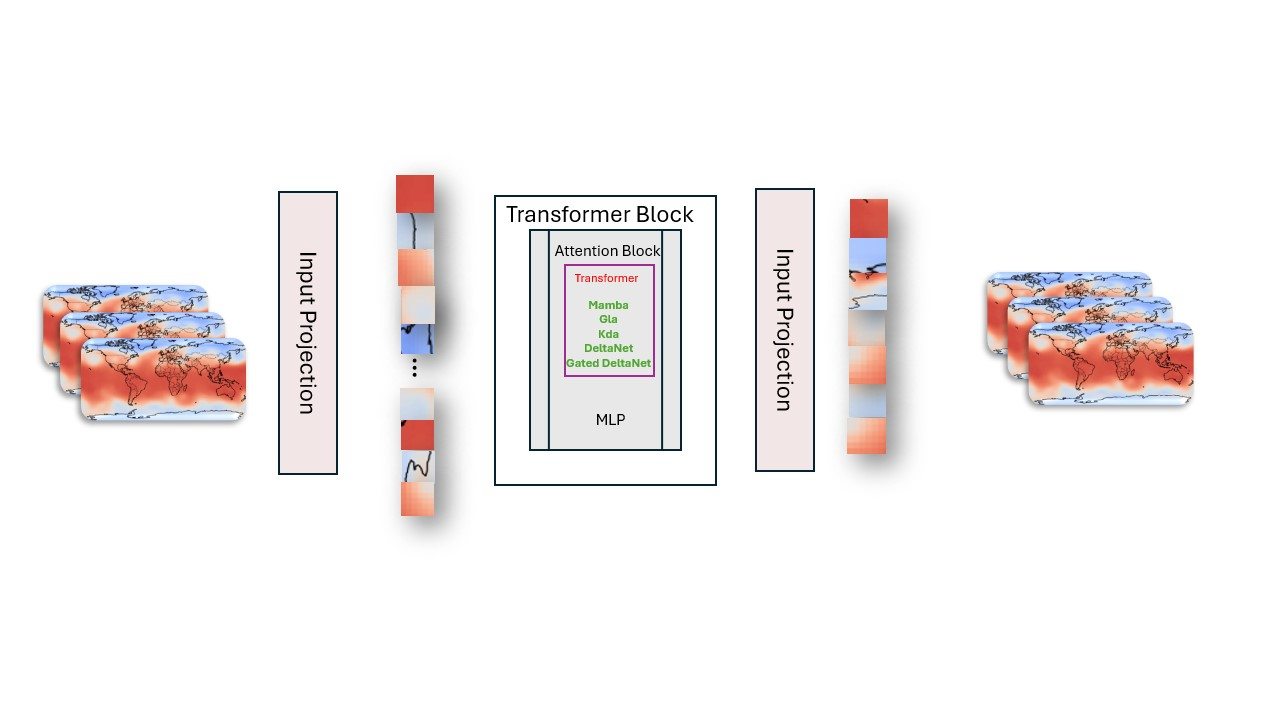
\includegraphics[width=0.9\textwidth]{figures/BlockDiagram.jpg}
    \caption{Unified model architecture for geopotential height forecasting. The attention backbone is interchangeable, enabling fair comparison across mechanisms.}
    \label{fig:architecture}
\end{figure}

\subsection{Training Objective}

We minimize the mean squared error between predictions and ground truth:
\begin{equation}
    \mathcal{L} = \frac{1}{T_{out} \cdot C \cdot H \cdot W} \sum_{t=1}^{T_{out}} \|y_t - \hat{y}_t\|_2^2
\end{equation}

Data is normalized per-level using pre-computed statistics from the training set:
\begin{equation}
    \tilde{x}_t^{(c)} = \frac{x_t^{(c)} - \mu^{(c)}}{\sigma^{(c)}}
\end{equation}
where $\mu^{(c)}$ and $\sigma^{(c)}$ are the mean and standard deviation for pressure level $c$.

%============================================================================
\section{Experimental Setup}
\label{sec:experiments}
%============================================================================

\subsection{Dataset}

We use NCEP/NCAR Reanalysis 1 geopotential height data~\cite{kalnay1996ncep}, which provides 6-hourly global atmospheric fields from 1948 to present. Our dataset covers:

\begin{itemize}
    \item \textbf{Spatial resolution:} $2.5° \times 2.5°$ latitude-longitude grid ($73 \times 144$ points)
    \item \textbf{Pressure levels:} 17 levels from 1000 hPa to 10 hPa
    \item \textbf{Primary evaluation level:} 500 hPa (standard benchmark in meteorology)
    \item \textbf{Temporal resolution:} 6-hourly snapshots
    \item \textbf{Train/validation split:} 90\% / 10\% chronological split
\end{itemize}

Table~\ref{tab:data_stats} summarizes the normalization statistics for selected pressure levels.

\begin{table}[t]
    \centering
    \caption{Normalization statistics for geopotential height at selected pressure levels.}
    \label{tab:data_stats}
    \begin{tabular}{lrrrr}
        \toprule
        \textbf{Level (hPa)} & \textbf{Mean (m)} & \textbf{Std (m)} & \textbf{Min (m)} & \textbf{Max (m)} \\
        \midrule
        1000 & 89.6 & 107.5 & -655.0 & 790.0 \\
        850 & 1,410.4 & 140.2 & 634.0 & 1,864.0 \\
        500 & 5,509.7 & 343.3 & 4,369.0 & 6,063.0 \\
        300 & 9,111.0 & 520.4 & 7,635.0 & 9,907.0 \\
        200 & 11,761.3 & 595.1 & 10,042.0 & 12,756.0 \\
        \bottomrule
    \end{tabular}
\end{table}

\subsection{Model Configurations}

To ensure fair comparison, all models are configured with approximately 340M parameters (Table~\ref{tab:model_configs}). Key architecture-specific parameters are set according to published recommendations for each model type.

\begin{table}[t]
    \centering
    \caption{Model configurations for the architecture comparison. All models have approximately 340M parameters.}
    \label{tab:model_configs}
    \begin{tabular}{lcccccc}
        \toprule
        \textbf{Model} & \textbf{Layers} & \textbf{Hidden} & \textbf{Heads} & \textbf{Head Dim} & \textbf{Params} \\
        \midrule
        Transformer & 24 & 1024 & 16 & 64 & $\sim$340M \\
        GLA & 24 & 1024 & 4 & 256 & $\sim$340M \\
        Gated DeltaNet & 21 & 1024 & 6 & 256 & $\sim$340M \\
        DeltaNet & 24 & 1024 & 8 & 128 & $\sim$340M \\
        Mamba2 & 48 & 1024 & -- & 64 & $\sim$340M \\
        KDA & 21 & 1024 & 6 & 256 & $\sim$340M \\
        \bottomrule
    \end{tabular}
\end{table}

\subsection{Training Configuration}

All models are trained using the \method{} framework with consistent hyperparameters:

\begin{itemize}
    \item \textbf{Input length ($T_{in}$):} 6 timesteps (36 hours)
    \item \textbf{Target length ($T_{out}$):} 1--24 timesteps (6--144 hours)
    \item \textbf{Batch size:} 8 per GPU
    \item \textbf{Optimizer:} AdamW with $\beta_1=0.9$, $\beta_2=0.999$, $\epsilon=10^{-15}$
    \item \textbf{Learning rate:} $3 \times 10^{-4}$ with cosine decay
    \item \textbf{Warmup steps:} 1,000
    \item \textbf{Total training steps:} 50,000
    \item \textbf{Gradient clipping:} Max norm 1.0
    \item \textbf{Precision:} Mixed precision (bfloat16)
\end{itemize}

\subsection{Evaluation Metrics}

We evaluate models using standard meteorological metrics:

\textbf{Root Mean Square Error (RMSE):}
\begin{equation}
    \text{RMSE} = \sqrt{\frac{1}{N}\sum_{i=1}^{N}(y_i - \hat{y}_i)^2}
\end{equation}

%\textbf{Mean Absolute Error (MAE):}
%\begin{equation}
%    \text{MAE} = \frac{1}{N}\sum_{i=1}^{N}|y_i - \hat{y}_i|
%\end{equation}

%\textbf{Anomaly Correlation Coefficient (ACC):}
%\begin{equation}
%    \text{ACC} = \frac{\sum_i (y_i - \bar{y})(\hat{y}_i - \bar{y})}{\sqrt{\sum_i (y_i - \bar{y})^2 \sum_i (\hat{y}_i - \bar{y})^2}}
%\end{equation}
%where $\bar{y}$ is the climatological mean. ACC $> 0.6$ is typically considered skillful forecast in operational meteorology.

\textbf{Computational Metrics:}
\begin{itemize}
    \item Training throughput (tokens/second)
    \item Peak GPU memory usage (GB)
    \item Inference latency (ms/sample)
\end{itemize}

\subsection{Baselines}

In addition to the attention mechanisms, we include:
\begin{itemize}
    \item \textbf{Persistence:} Predict $\hat{y}_t = x_{T_{in}}$ (last input frame)
    \item \textbf{Climatology:} Predict $\hat{y}_t = \bar{y}$ (training set mean)
\end{itemize}

%============================================================================
\section{Results}
\label{sec:results}
%============================================================================

\todoremark{Results to be added after experiments}

\subsection{Main Comparison}

Table~\ref{tab:main_results} presents the forecasting performance of all architectures at 24-hour lead time on 500 hPa geopotential height.

\begin{table}[t]
    \centering
    \caption{Forecasting performance on 500 hPa geopotential height at 24-hour lead time. Best results in \textbf{bold}, second best \underline{underlined}.}
    \label{tab:main_results}
    \begin{tabular}{lccccc}
        \toprule
        \textbf{Model} & \textbf{RMSE (m)} & \textbf{MAE (m)} & \textbf{ACC} & \textbf{Tokens/s} & \textbf{Memory (GB)} \\
        \midrule
        Persistence & -- & -- & -- & -- & -- \\
        Climatology & -- & -- & -- & -- & -- \\
        \midrule
        Transformer & -- & -- & -- & -- & -- \\
        GLA & -- & -- & -- & -- & -- \\
        Gated DeltaNet & -- & -- & -- & -- & -- \\
        DeltaNet & -- & -- & -- & -- & -- \\
        Mamba2 & -- & -- & -- & -- & -- \\
        KDA & -- & -- & -- & -- & -- \\
        \bottomrule
    \end{tabular}
\end{table}

\subsection{Forecast Horizon Analysis}

\begin{figure}[t]
    \centering
    \begin{subfigure}[t]{0.48\textwidth}
        \centering
        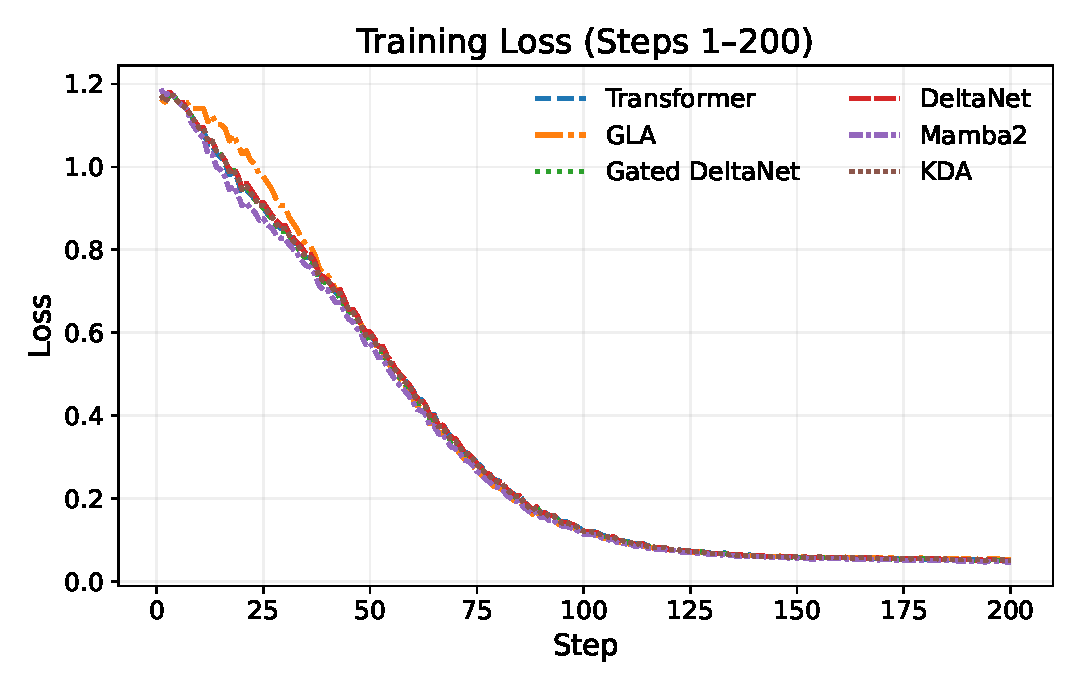
\includegraphics[width=\textwidth]{figures/loss_train_200steps.pdf}
        \caption{Training loss (steps 1--200).}
    \end{subfigure}
    \hfill
    \begin{subfigure}[t]{0.48\textwidth}
        \centering
        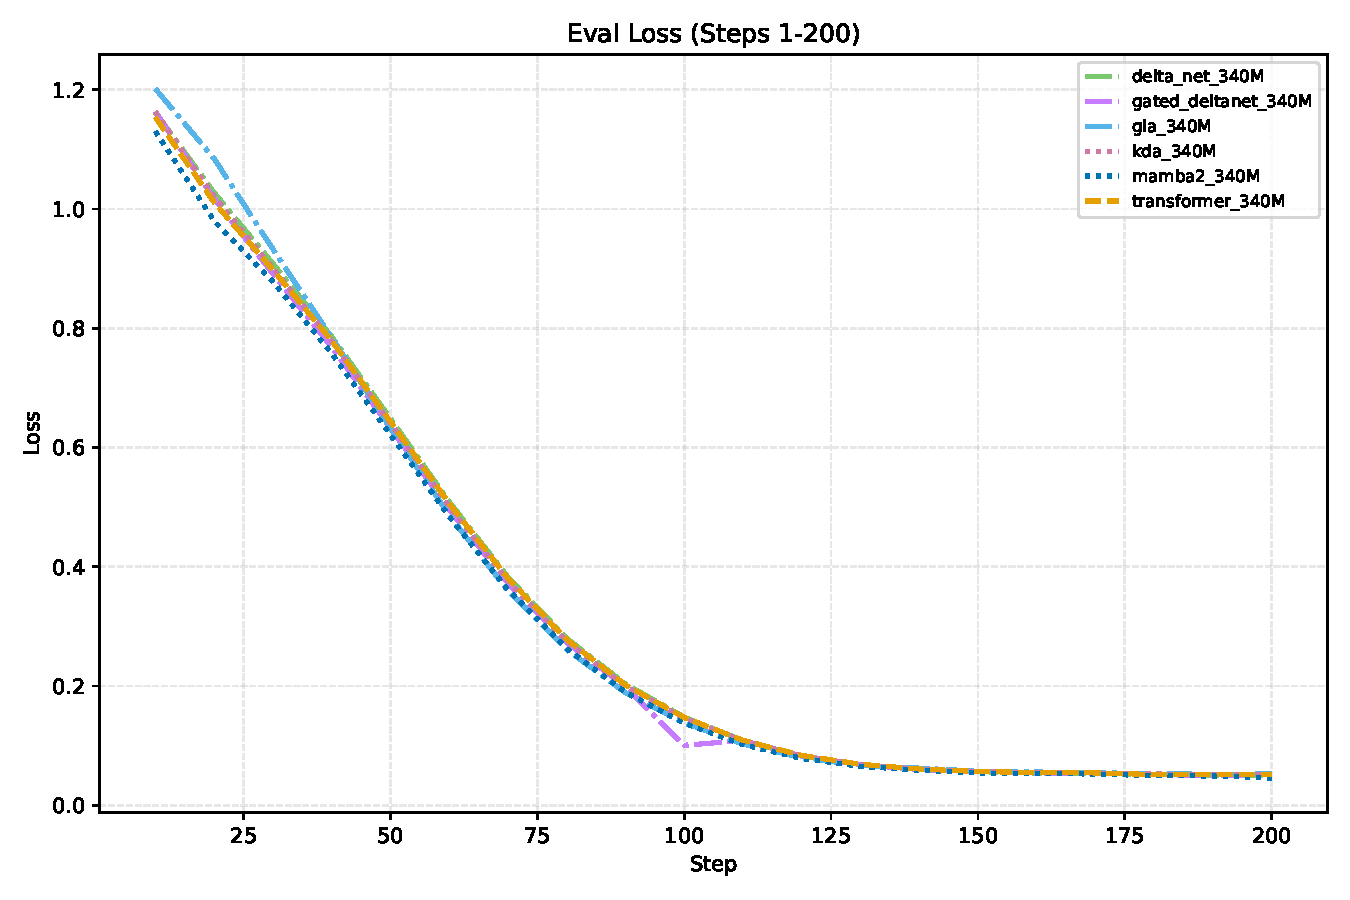
\includegraphics[width=\textwidth]{figures/loss_eval_200steps.pdf}
        \caption{Eval loss (steps 1--200).}
    \end{subfigure}
    \caption{Training and evaluation loss on HGT over the first 200 steps for Transformer, GLA, DeltaNet, Gated DeltaNet, KDA, and Mamba2.}
    \label{fig:loss-train-eval-200}
\end{figure}

Here’s the grouped figure snippet for throughput + memory scaling (read‑only, no edits):
\begin{figure}[t]
    \centering
    \begin{subfigure}[t]{0.48\textwidth}
        \centering
        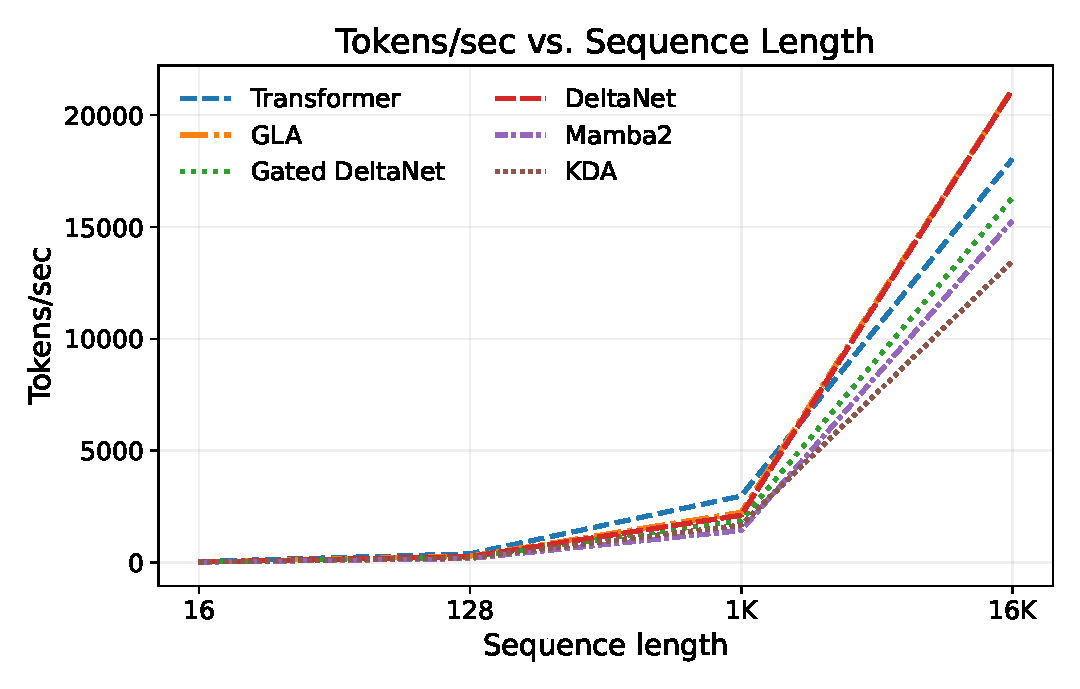
\includegraphics[width=\textwidth]{figures/throughput_scaling.pdf}
        \caption{Tokens/sec vs. sequence length.}
    \end{subfigure}
    \hfill
    \begin{subfigure}[t]{0.48\textwidth}
        \centering
        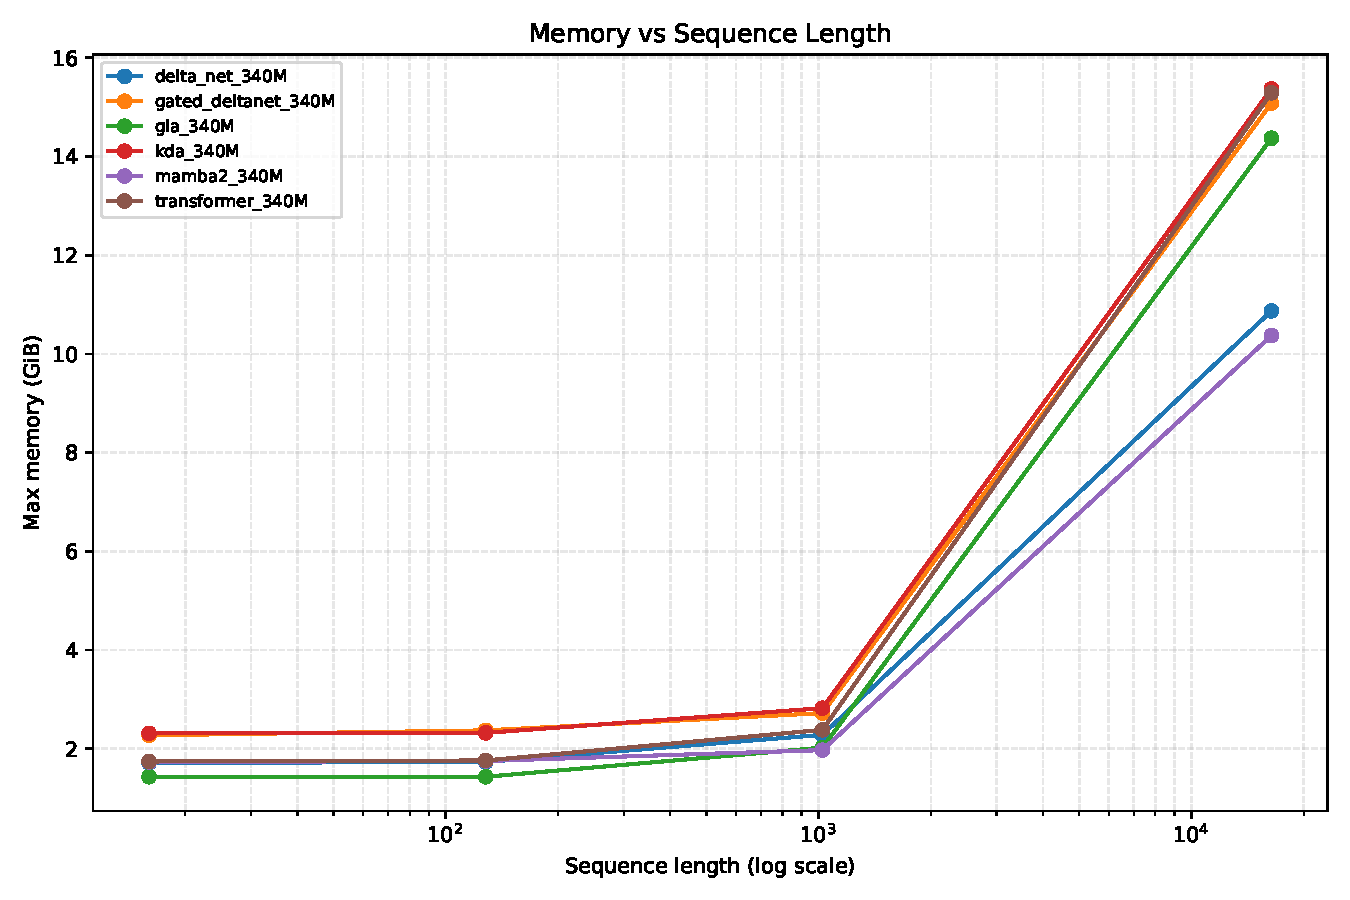
\includegraphics[width=\textwidth]{figures/memory_scaling.pdf}
        \caption{Memory vs. sequence length.}
    \end{subfigure}
    \caption{Throughput and memory scaling on HGT at sequence lengths 8K, 32K, and 131K.}
    \label{fig:throughput-memory}
\end{figure}

%\todoremark{Add figure showing RMSE vs lead time for all models}

\subsection{Computational Efficiency}

%\todoremark{Add throughput and memory comparison}

%============================================================================
\section{Discussion}
\label{sec:discussion}
%============================================================================

\todoremark{Discussion to be added after experiments}

%============================================================================
\section{Conclusion}
\label{sec:conclusion}
%============================================================================

We presented a systematic comparison of linear attention architectures for geopotential height forecasting. Our experiments on NCEP reanalysis data demonstrate that [findings to be added]. The \method{} framework enables efficient training of these models with distributed data parallelism and is released as open source to facilitate future research.

\textbf{Limitations and Future Work:} Our study focuses on single-variable forecasting at fixed spatial resolution. Future work will explore multi-variable prediction, higher resolution data, and longer forecast horizons.

%============================================================================
% Bibliography
%============================================================================

\bibliographystyle{splncs04}
\bibliography{references}

\end{document}
